\documentclass[titlepage,a4paper]{jsarticle}
\usepackage{../../../sty/import}% 各種パッケージインポート
\usepackage{../../../sty/title}% タイトルページの変更

%% タイトルページの変数
% レポートタイトル
\title{中間レポート}
% 提出日
\expdate{\today}
% 科目名
\subject{統計的信号処理特論}
% 分野
\class{情報経営システム工学分野}
% 学年
\grade{M1}
% 学籍番号
\mynumber{24336488}
% 記述者
\author{本間三暉}

\begin{document}
% titleページ作成
\maketitle
%% テーマ
% 主成分分析または線形判別
% リワーク後ブリーズにおける対戦環境
% コンペ,レディアント,ブリーズ,コントローラー,var12.06,4/20時点
% 真剣にやってそうな人が多そうだから,最上位帯なのでスマーフなどハズレ値を弾けそう,リワークされてかなり対戦環境に変化があったため，またすべてのキャラがでるので,リワークの影響を一番受けているであろうロールなので,データ取得時点のデータが動かない最新のデータ(4/20時点の最新は12.07)
\section{はじめに}\label{first}
  私は，オンラインFPSゲームであるValorantの対戦環境について主成分分析を行う．
今回分析するにあたって，実際のキャラクターの性能とマップの相性を正確に把握するためいくつかの条件を設けた．
まず，分析対象を最上位のランク帯であるレディアントに限定する．
オンラインゲームには往々にしてサブ垢やスマーフと呼ばれる実際の実力より低いランク帯でプレイするプレイヤーが存在する．
このようなプレイヤーは，自分で完結し試合を破壊できるキャラクターを選ぶ傾向があるため，分析対象を最上位のランク帯に限定することで，このようなプレイヤーの影響を減らすことができると考えたからである．

  また，分析対象のマップは2026年1月に1年半ぶりにマップローテーションに追加されたブリーズ\cite{パッチノート}である．
このブリーズというマップは，以前マップローテーションにあったときと比べ，いくつかの変更が行われた．
この変更によって対戦環境が大きく変化したと考えられる．

  次に，分析対象のキャラクターはコントローラーというロールのキャラクターに限定する．
コントローラーは，相手の視界を遮る能力を持つキャラクターで，以前のブリーズでは一つのキャラクターに人気が集中していたが，
リワークによってそれ以外のキャラクターにも日の目が当たるようになったからである．
プロシーンを見ても，カーテン型のスモークを出せるキャラクターしか出ていなかった状態から，他のマップと同様に一般的な丸いスモークしか出せないキャラクターも出るようになっており，
リワークの影響を一番受けているロールであると考えられるからである．

最後に，分析対象のデータは2026年5月11日時点で，内容が確定している内の最新データであるVar.12.07を使用する．

\section{データの取得}
  データはValorantの統計サイトであるOP.GG\cite{opgg}から取得した．
このサイト内で章\ref{first}で述べた条件を満たす条件で内容を絞ったキャラクター名，勝率，使用率，K/Dである．

  勝率はそのキャラクターを使用した試合のうち，勝利した試合の割合を表す．基本的には，同じ互いに同じキャラクターを使用している場合勝率は50\%になるはずである．

  使用率はそのキャラクターが使用された試合の割合を表す．
使用率が高いほどそのキャラクターが人気であることを表していて，5v5のゲームであるValorantにおいては最大値が20\%になると考えられる．

  K/Dはキル数をデス数で割った値で，この値が大きいほどキル数が多くデス数が少ないことを表す．
Valorantにおいては，コントローラーはキルを取っていないのにもかかわらずスキルで相手を動かすことで勝利に貢献することが多いため，
K/Dが高いからといって必ずしも勝っているとは限らない．

取得したデータを表\ref{data}に示す．
\begin{table}[H]
\centering
\caption{OP.GGから取得したデータ}
\label{data}
  \begin{tabular}{l|llll}\hline
  キャラクター名 & 勝率[\%] & 使用率[\%] & K/D &  \\\hline\hline
  ヴァイパー   & 51.62\% & 8.79\% & 1.09 &  \\
  クローヴ    & 56.18\% & 4.01\% & 1.03 &  \\
  アストラ    & 47.27\% & 3.85\% & 1.05 &  \\
  ミクス     & 53.47\% & 3.03\% & 1.03 &  \\
  オーメン    & 48.08\% & 1.56\% & 1.12 &  \\
  ハーバー    & 45.00\% & 0.90\% & 1.13 &  \\
  ブリムストーン & 44.44\% & 0.41\% & 0.89 & \\\hline
  \end{tabular}
\end{table}
\section{主成分分析}
  表\ref{data}のデータをもとに主成分分析を行った．
その分析結果を表\ref{pca}に示す．
また，主成分係数を図\ref{coef}に示す．
さらに，主成分スコアを図\ref{score}に示す．
\begin{table}[H]
\centering
\caption{主成分分析の結果}
\label{pca}
% tabler環境の挿入
\begin{tabular}{l|lll}\hline
        & 第一主成分  & 第二主成分  & 第三主成分 \\\hline\hline
ヴァイパー   & -2.23 & -1.08 & 0.18     \\
クローヴ    & -1.12 & 0.98  & 0.51     \\
アストラ    & 0.07  & -0.43 & -0.14    \\
ミクス     & -0.01 & 0.7   & -0.12    \\
オーメン    & 0.45  & -0.14 & -0.52    \\
ハーバー    & 0.11  & 0.41  & -0.37    \\
ブリムストーン & 2.72  & -0.45 & 0.46    \\\hline
\end{tabular}
\end{table}

\begin{table}[H]
\centering
\caption{主成分係数の結果}
\label{coef}
% tabler環境の挿入
\begin{tabular}{l|lll}\hline
            & 第一主成分 & 第二主成分 & 第三主成分 \\\hline\hline
勝率{[}\%{]}  & -0.52 & 0.82  & 0.24  \\
使用率{[}\%{]} & -0.58 & -0.55 & 0.6   \\
K/D         & -0.62 & -0.17 & -0.76\\\hline
\end{tabular}
\end{table}

\begin{table}[H]
\centering
\caption{主成分分析の固有値・寄与率・累積寄与率の結果}
\label{score}
% tabler環境の挿入
\begin{tabular}{l|lllll}\hline
主成分 &固有値 &寄与率 & 累積寄与率 \\\hline\hline
第1主成分 &2.3102 &0.7701 & 0.7701    \\
第2主成分 &0.5325 &0.1775 & 0.9475    \\
第3主成分 &0.1574 &0.0525 & 1.0000      \\\hline
\end{tabular}
\end{table}

主成分分析の結果をフラフにしたものを図\ref{fig}に示す．
\begin{figure}[H]
\centering
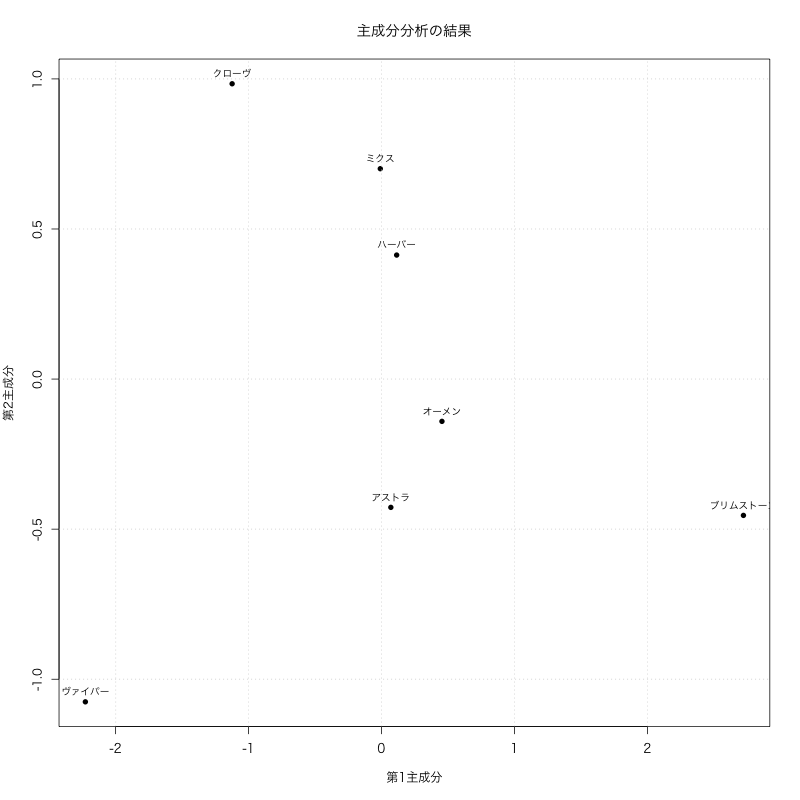
\includegraphics[width=0.8\textwidth]{other/valo_result_plot.png}
\caption{主成分分析の結果}
\label{fig}
\end{figure}
\section{考察}
表\ref{coef}から，第一主成分ではすべての変数が同方向に寄与していることがわかる．
これは，強力なキャラクターほどプレイヤーから広く使用され，さらにK/Dも高くなりやすいという，ゲーム内のキャラクター選択傾向を反映している可能性がある．
また，本分析では勝率，使用率，K/Dが高いキャラクターほど第一主成分が負方向に位置した．
このことから，第一主成分はキャラ性能や使いやすさを表す軸であると考えられる．
ゲームプレイの観点ではトロール度，マニアック度や味方に理解されにくい度合いを反映している可能性もある．

第二主成分では，勝率が正方向，使用率とK/Dが負方向に寄与していた．
また，第一主成分と比べてK/Dの係数が小さいことから，第二主成分では特に勝率と使用率の影響が大きいことがわかる．
これは，「勝率は高いが積極的には使用されていないキャラクター」を表している可能性がある．

Valorantにおけるコントローラーは，直接キルを取ることよりも，スモークによる視界制御によってチーム全体を支援する役割が重要である．
そのため，K/Dが高くなくても勝率が高くなるキャラクターが存在すると考えられる．
また，味方構成の都合上，本来使いたいキャラクターではなくチームバランスのためにコントローラーを選択する場合も存在する．
このことから，第二主成分は合わせピック傾向や，勝つためには必要だが積極的には使われにくいキャラクターを表す軸であると考えられる．

キャラ別に見ることで，なぜこのような結果になったのかを考察する．

ヴァイパーは第一主成分，第二主成分ともに最も低い値を取っていた．
第一主成分は総合性能や汎用性を表していることから，ヴァイパーは扱いやすく，多くのプレイヤーから安定して使用されているキャラクターであると考えられる．
実際に，ブリーズではヴァイパーのようなカーテン型スモークが非常に強力であり，マップのリワーク前から継続して高い使用率を持っていた．
そのため，プレイヤーが新しくセットアップを覚え直す必要が少なく，この結果はブリーズにおけるヴァイパーの高いマップ適性と整合的である．

クローヴは第一主成分が2番目に低く，第二主成分が最も高い値を取っていた．
第二主成分は，勝率が高く，使用率が低い方向を表している．
このことから，クローヴは性能自体は高いものの，マップ適性や役割上の理由から，積極的には選択されにくいキャラクターである可能性がある．

一方で，クローヴは撃ち合い性能が高く，デュエリストに近い感覚で使用できるキャラクターである．
そのため，味方構成の都合でコントローラーが必要になった場合に，キャラクター性能や扱いやすさから選択されやすいと考えられる．
特に，今回分析対象としたレディアント帯では，プレイヤー自身の撃ち合い能力が高いと考えられるため，クローヴのような撃ち合い寄りのコントローラーが選択されやすい可能性がある．

このような結果から，第一主成分は総合性能や汎用性を表す軸，第二主成分は合わせピック傾向や，勝つためには必要だが積極的には使用されにくいキャラクターを表す軸であると考えられる．

\section{AI使用箇所}
  今回のレポートでは，主成分分析を行う際のソースコードの生成でAIを使用した．
  また，ざっくりとレポート内にどのような項目があるとわかりやすいかをAIに聞いた．
  更に，完成したレポートを添削してもらい，結果や考察の内容が不足していないかを確認してもらい，アドバイスをもらった．
% 参考文献
\begin{thebibliography}{99}
\bibitem{授業資料} 統計的信号処理特論 授業資料
\bibitem{パッチノート} VALORANT パッチノート 12.00\\
\url{https://playvalorant.com/ja-jp/news/game-updates/valorant-patch-notes-12-00/}
\bibitem{opgg} Valorant Stats - VALORANT.OP.GG \url{https://op.gg/ja/valorant/statistics}
\end{thebibliography}

\end{document}